% ClassLink UML figures — ready-to-paste \input{} block for the report.
% Assumes main.tex is at the repository root, so paths below are relative
% to the repo root (docs/uml/png/...). Requires \usepackage{graphicx} and
% \usepackage{float} (for the [H] placement specifier) in the preamble.

\begin{figure}[H]
    \centering
    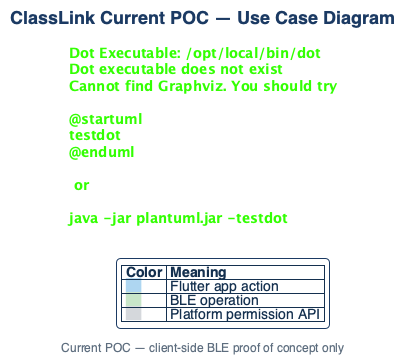
\includegraphics[width=0.95\textwidth]{docs/uml/png/01-use-case-current-poc.png}
    \caption{ClassLink current POC use case diagram, showing teacher and student actions implemented in the BLE proof of concept.}
    \label{fig:uml-use-case}
\end{figure}

\begin{figure}[H]
    \centering
    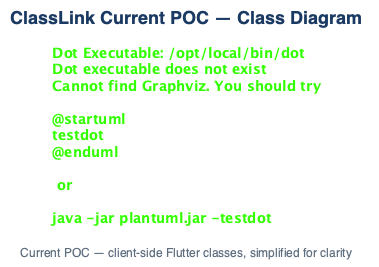
\includegraphics[width=0.95\textwidth]{docs/uml/png/02-class-current-poc.png}
    \caption{ClassLink current POC class diagram, showing the client-side Flutter classes responsible for advertising, scanning, proximity evaluation and check-in.}
    \label{fig:uml-class}
\end{figure}

\begin{figure}[H]
    \centering
    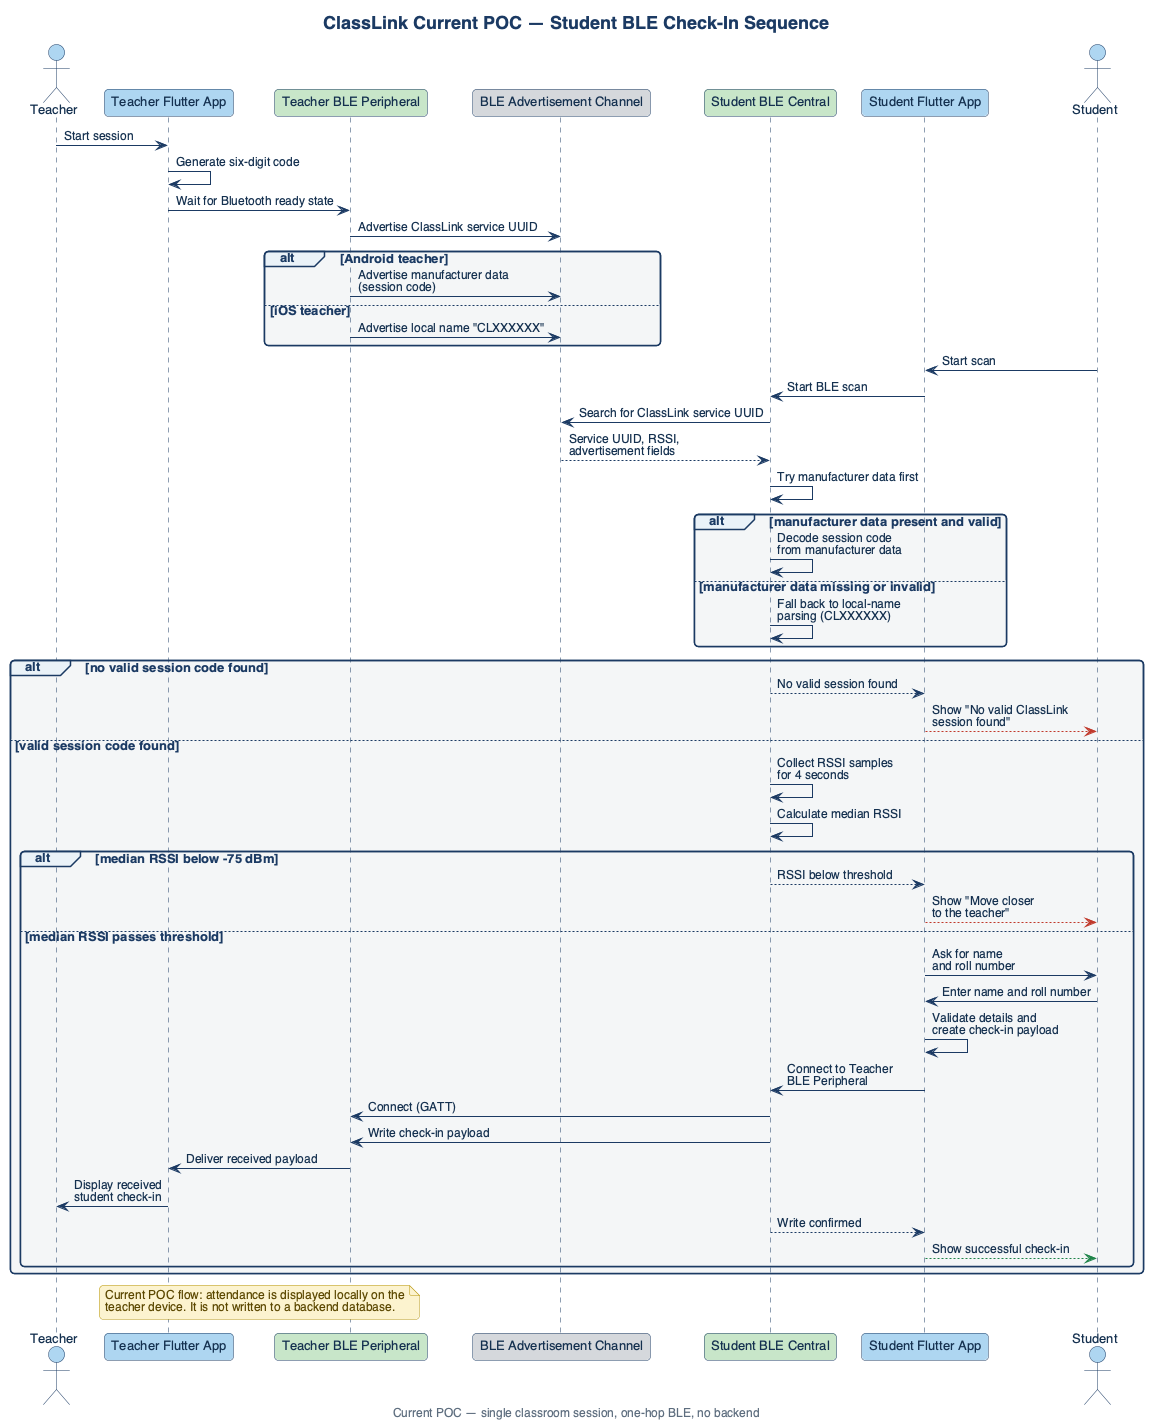
\includegraphics[width=\textwidth]{docs/uml/png/03-sequence-student-checkin.png}
    \caption{ClassLink current POC sequence diagram for a student BLE check-in, including the Android manufacturer-data path, the iOS local-name fallback, invalid-code handling and weak-RSSI rejection.}
    \label{fig:uml-sequence}
\end{figure}

\begin{figure}[H]
    \centering
    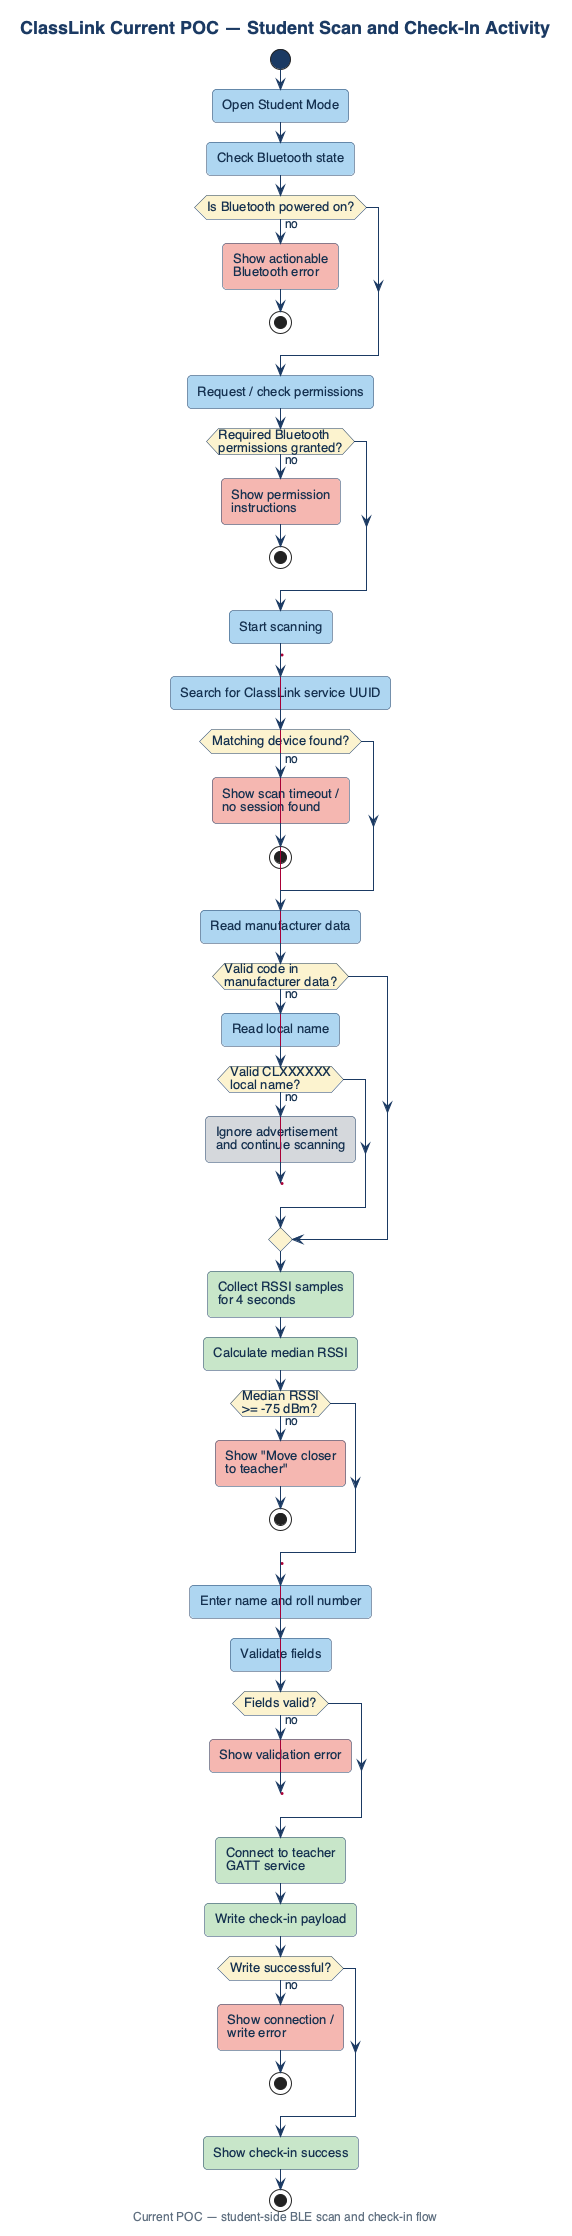
\includegraphics[width=\textwidth]{docs/uml/png/04-activity-student-scan.png}
    \caption{ClassLink current POC activity diagram for the student scan and check-in flow, from permission checks through RSSI evaluation to GATT write confirmation.}
    \label{fig:uml-activity}
\end{figure}

\begin{figure}[H]
    \centering
    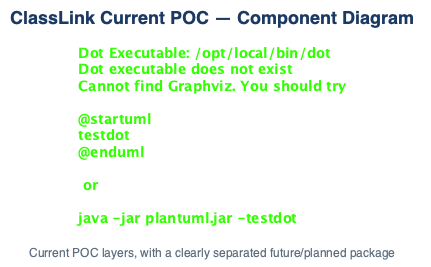
\includegraphics[width=0.95\textwidth]{docs/uml/png/05-component-current-poc.png}
    \caption{ClassLink current POC component diagram, showing the Flutter presentation, application, BLE communication, native platform and development/quality layers, with the planned backend shown separately as not implemented.}
    \label{fig:uml-component}
\end{figure}

\begin{figure}[H]
    \centering
    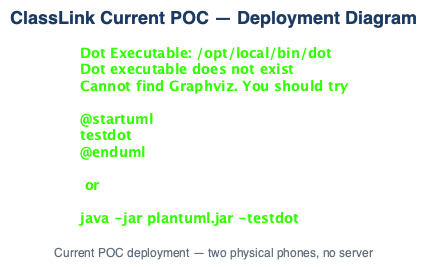
\includegraphics[width=0.95\textwidth]{docs/uml/png/06-deployment-current-poc.png}
    \caption{ClassLink current POC deployment diagram, showing the two physical phones, the private source repository and the build artifacts used for testing, with the planned cloud deployment shown separately as not implemented.}
    \label{fig:uml-deployment}
\end{figure}

\begin{figure}[H]
    \centering
    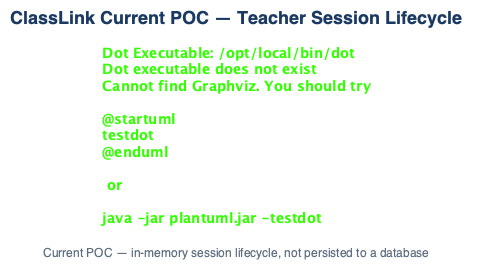
\includegraphics[width=0.80\textwidth]{docs/uml/png/07-state-session-lifecycle.png}
    \caption{ClassLink current POC state diagram for the teacher session lifecycle, from session start through advertising, check-in reception and session close.}
    \label{fig:uml-state}
\end{figure}
